\chapter{Bots basados en secuencias de acciones} \label{cap:bots-secuencia-acciones}
En primer lugar y una vez decididos nuestros dos frameworks de partida, fue necesaria la integración entre el código de Pac-Man y JECO para poder empezar a realizar experimentos.

\section{Integración de Ms. Pac-Man y JECO}
\begin{figure}[H]
\centering
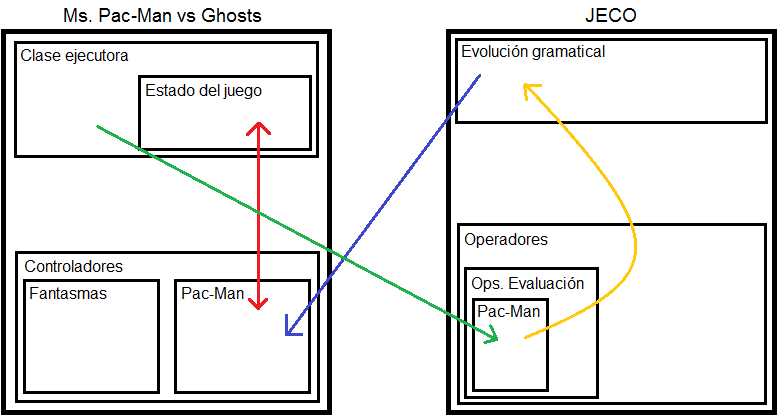
\includegraphics[width=\textwidth]{integracion-jeco-pacman}
\end{figure}
\begin{itemize}
\item Flecha azul: JECO evoluciona individuos (en la primera generación son aleatorios) y transmite su fenotipo al framework de Pac-Man, para ser evaluados.

\item Flecha roja: El controlador de Pac-Man suministra movimientos a la clase ejecutora, al tiempo que la clase ejecutora transmite información necesaria al controlador para que este pueda determinar qué movimientos hacer.

\item Flecha verde: El framework de Pac-Man transmite a una función de evaluación especializada para Pac-Man en JECO la información de la partida (en primer lugar empezamos transmitiendo únicamente la puntuación obtenida).

\item Flecha amarilla: La función de evaluación para Pac-Man traduce la información resultante de la partida a un fitness, que es transmitido al proceso de evaluación gramatical. El individuo evaluado adquiere un fitness y en función del mismo se condiciona la siguiente generación (junto a los resultados del resto de individuos).
\end{itemize}

Debido a que JECO persigue encontrar individuos con el fitness más bajo posible (minimización), tenemos la necesidad de emplear fitness en los que se considere mejor el menor o adaptarlo a maximización. Optamos por lo primero, y empleamos como fitness inicial:
\begin{equation}
f = 100000 - score
\end{equation}
donde $score$ es la puntuación total que conseguimos y $100000$ es una cota máxima a dicha puntuación.


\section{Idea general}
Empezamos por plantearnos los objetivos más sencillos e indispensables:
\begin{itemize}
\item Gramáticas evolutivas mono-objetivo.
Un solo thread.

\item Una sola función de fitness que tuviera únicamente en cuenta los puntos conseguidos (Recibiendolos JECO tras cada evaluación del árbol de derivación obtenido en Pac-Man).

\item Uso de una gramática que solo permitiese generar programas en forma de cadena de movimientos simples (\textbf{\texttt{U D L R}}) como una sucesión de caracteres.

\item Un generador de trazas minimalista para registrar los fenotipos que producían una mejora del fitness durante la ejecución.
\end{itemize}

Partiendo de un sistema de evolución gramatical que devolvía árboles de derivación en forma de cadenas de caracteres, la idea inicial fue encapsular tanto acciones como observadores del estado del juego dentro de dichas cadenas, que contendrían de manera prefijada las acciones a realizar o evaluar por el controlador de Pac-Man, repitiéndose en un bucle la evaluación de los caracteres de la cadena desde el principio de la misma al llegar al final. Dicha cadena-programa puede verse como un autómata en las que las transiciones son la evaluación de un carácter y paso al siguiente.

\section{Un primer bot}
La primera versión de autómata conseguido encadenaba los distintos movimientos posibles (\texttt{Arriba, Abajo, Derecha, Izquierda}, \textbf{\texttt{U D L R}} respectivamente) pertenecientes a un alfabeto inicial que más tarde fuimos ampliando y mejorando durante la implementación.
 
El controlador de Pac-Man generaba una transición en el autómata secuencialmente al tiempo que este le proporcionaba el movimiento asociado al estado al que transitaba, volviendo el autómata al estado inicial cuando finalizaba la cadena de caracteres definidos por la gramática. El fundamental problema de este sistema es que el bot no tiene en cuenta el estado de juego, viéndose obligado a realizar acciones de la secuencia que tal vez sean contraproducentes.
 
Por ejemplo, para una de nuestras más sencillas gramáticas de partida:
\begin{lstlisting}[frame=single, breaklines=no, basicstyle=\fontsize{10}{11}\ttfamily]
    <mov> ::= <mov> U  | 
              <mov> D  | 
              <mov> R  | 
              <mov> L  |
              U | 
              D | 
              R |
              L
\end{lstlisting}

Una derivación gramatical válida podría ser: ``\textbf{\texttt{U R D L}}'', que podría verse como un autómata con la siguiente forma \cite{jflapPage}:
\begin{figure}[H]
\centering
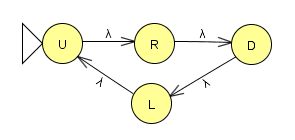
\includegraphics[width=8cm]{jflapo}
\end{figure}

El controlador consume un símbolo tras otro transitando al siguiente estado del autómata al mismo tiempo, traduciéndose en este caso en un comportamiento que lleva a Pac-Man a intentar dar vueltas en sentido horario.
 
Sorprendentemente únicamente con esto, al ser los laberintos siempre los mismos, conseguía hacer algunos puntos antes de ser aniquilado por los fantasmas, pese a la precariedad del método. Lo relevante en este punto era que teníamos una primera integración que funcionaba.
 
A continuación se muestra el resultado de uno de los primeros experimentos realizados, con tamaño de población 100, 50 generaciones, una evaluación por individuo, selección por Torneo Binario, cruce monopunto con 60\% de probabilidad de cruce e \textit{Integer flip mutation} con 10\% de probabilidad de mutación. El controlador de fantasmas era \textit{Starter ghosts} (nuestro bot aún no tenía ninguna oportunidad contra \textit{Legacy}).
\begin{table}[H]
\centering
\begin{tabular}{cc}
\hline
\textbf{Fenotipo} & \textbf{Puntos (avg)} \\ \hline
\texttt{LLDLDRLD}          & 2480                  \\ \hline
\end{tabular}
\end{table}

\section{Incorporando condicionales y acciones de alto nivel}
Para dotar al autómata de capacidad de decisión que tuviera en cuenta el estado del juego en el que se encontraba el bot, incluimos \textbf{símbolos condicionales}, que siempre iban precedidos del símbolo ``\texttt{?}''. A su vez el símbolo ``\texttt{?}'' siempre iba precedido de un carácter que representaba la condición a evaluar.
Si una condición evaluada resultaba cierta, se realizaba la \textbf{acción} que definía el carácter ubicado a continuación del de la condición. Si no, se omitía. 

\blankline

La versión final disponía de evaluaciones y acciones de alto nivel especificados por la cadena de instrucciones del autómata, cuyo alfabeto era el siguiente:
\begin{table}[H]
\centering
\begin{tabular}{ccc}
\hline
\textbf{Char} & \textbf{Tipo de símbolo} & \textbf{Comportamiento}                     \\ \hline
P             & condicional              & Condicional de fantasma no comestible cerca \\
B             & condicional              & Condicional de fantasma comible cerca       \\
H             & acción                   & Huir                                        \\
E             & acción                   & Comer pill                                  \\
W             & acción                   & Comer powerpill                             \\
F             & acción                   & Comer fantasma                              \\ \hline
\end{tabular}
\end{table}

La gramática diseñada para hacer uso de este lenguaje, tenía la siguiente forma:
\begin{lstlisting}[frame=single, breaklines=no, basicstyle=\fontsize{10}{11}\ttfamily]
    <expr>   ::= ? <cond> <expr> | <action> <expr> | <action>
    <cond>   ::= P | B
    <action> ::= H | E | W | F
\end{lstlisting}

\subsection{Fenotipos producidos}
En bots producidos por esta implementación a veces se aprecia un atisbo de primera inteligencia muy primitiva, así como los habituales intrones o fragmentos de programa inútiles.
 
Los siguientes fenotipos fueron obtenidos tras experimentos con tamaño de población 100, 50 generaciones, una evaluación por individuo, selección por Torneo Binario, cruce monopunto con 60\% de probabilidad de cruce e \textit{Integer flip mutation} con 10\% de probabilidad de mutación. Los fantasmas siguen siendo \textit{Starter ghosts} en esta etapa, dados los malos resultados obtenidos contra fantasmas \textit{Legacy}.
\begin{table}[H]
\centering
\begin{tabular}{cc}
\hline
\textbf{Fenotipo} & \textbf{Puntos (avg)} \\ \hline
\texttt{E?P?PH}          & 6580                  \\
\texttt{?B?PE?BHEHE}          & 7000                  \\ \hline
\end{tabular}
\end{table}

Como ejemplo, la traducción a pseudocódigo del primer programa sería lo siguiente:
\begin{lstlisting}[frame=single, breaklines=no, basicstyle=\fontsize{10}{11}\ttfamily]
    MIENTRAS (true)
        Ir hacia la pill más cercana
        SI (fantasma no comible cerca) ENTONCES
            SI (fantasma no comible cerca) ENTONCES
                Huir del fantasma no comible más cercano
            FIN SI
        FIN SI
    FIN MIENTRAS
\end{lstlisting}

Que se traduce en ir siempre hacia la pill más cercana, salvo que haya un fantasma no comible cerca de Pac-Man, en cuyo caso se aleja de él. Se aprecia una doble evaluación consecutiva de lo mismo que no aporta nada: Un problema típico en programación genética. 

\blankline

Resulta destacable el descubrimiento por parte de los bots generados mediante este sistema de la variable ``\textit{Global reversal}'', que en cada movimiento asigna a los fantasmas una probabilidad aleatoria muy baja de darse todos la vuelta.
 
Los fenotipos consistentes en comer pills y huir cuando haya un fantasma cerca, producen una estrategia en la que el bot de Pac-Man huye a la vez que agrupa la mayoría de fantasmas detrás de él. Cuando ocurre el susodicho \textit{Global reversal}, los fantasmas cambian su dirección a la opuesta, y dado que no pueden cambiarla de nuevo salvo que ocurra otro global reversal y las distancias son calculadas teniendo esta limitación en cuenta, todos pasan a estar ``lejos'' de Pac-Man y este puede comer pills con seguridad.
\begin{figure}[H]
\centering
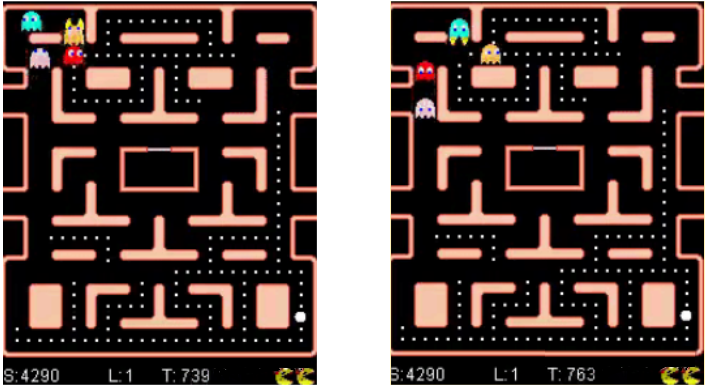
\includegraphics[width=0.8\textwidth]{global-reversal}
\caption{\textit{Global reversal} de los fantasmas.}
\end{figure}

\section{Limitaciones}
Tal como esperábamos, el empleo de este ingenuo autómata tiene varias limitaciones.
 
El funcionamiento de nuestros condicionales permitía una sola condición, es decir, no nos permitían evaluar varias premisas (usando operadores lógicos binarios y/o unarios) salvo mediante el encadenamiento de condicionales (\texttt{if}). 
Tampoco teníamos la posibilidad de emplear una segunda acción que solo se ejecutase en caso de no cumplirse el condicional, a modo ``\texttt{else}''. Además, solo se realizaba una acción en el consecuente, en lugar de poder realizar una serie de acciones. 
 
Otra limitación era la imposibilidad de construir estrategias con continuidad temporal debido a la ejecución de la cadena de instrucciones de forma lineal, dado que esta era única para toda la ejecución y simplemente se volvía a empezar por el principio tras llegar al final.
 
Además, este funcionamiento en forma de bucle que repite la misma secuencia de acciones podía provocar muy fácilmente la ejecución de una acción sin sentido en el contexto en el que el juego se encontraba en determinado momento.
 
Previamente decidimos comprobar si era posible adaptar el autómata con el que contábamos en ese momento de forma que se solventase los problemas descritos.
 
Para dicha prueba, introdujimos un nuevo estado de huida (similar a un estado trampa, pero con una vía de salida), en el que se entraba en caso de encontrarse algún fantasma (comible) por debajo de un radio de peligro. 
En este estado de huida se codificaba un comportamiento, en alto nivel y ajeno al funcionamiento normal del autómata, en el que permanecía hasta que Pac-Man estuviera fuera de la distancia de peligro. Tras estar fuera de peligro, el bot salía del estado de huida y seguía ejecutando la cadena de instrucciones dada por el autómata en el punto en el que se encontraba antes de entrar al estado de huida.
\begin{figure}[H]
\centering
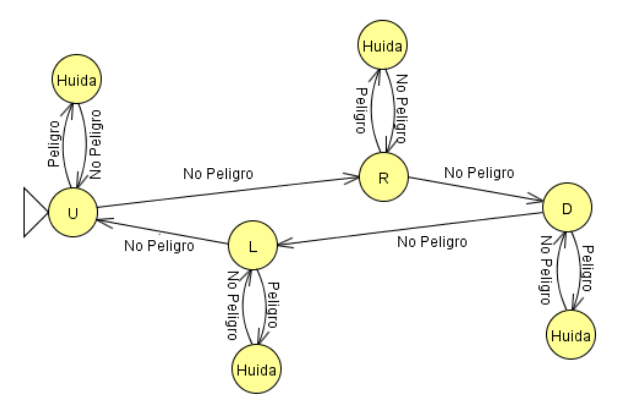
\includegraphics[width=0.8\textwidth]{prueba-automata}
\caption{Ejemplo de autómata que usa el estado Huida.}
\end{figure}

A través de esta prueba comprobamos que la escalabilidad del autómata no era realista, ya que suponía la codificación de eventos cada vez más complejos de gestionar debido a la aparición de conflictos con los ya introducidos a la hora de controlar las transiciones.
 
Llegados a este punto y con esos problemas, considerábamos seriamente la posibilidad de realizar una nueva implementación alejada del sistema de autómatas de movimientos concatenados.
